Το μοντέλο ψευδο-μόνιμης κατάστασης (\textit{QSS}) που περιγράφτηκε στα προηγούμενα
κεφάλαια δεν διαθέτει μοντέλο οδηγού και, ως εκ τούτου, εκτελεί κάθε γύρο στο όριο του
διαγράμματος επιδόσεων. Στην πραγματικότητα, ο οδηγός μειώνει σκόπιμα την εκμετάλλευση
του διαγράμματος. Η ανάπτυξη ενός πλήρους βελτιστοποιητή που να
αναπαράγει αυτή τη συμπεριφορά ξεφεύγει από το εύρος της παρούσας εργασίας. Αντ' αυτού,
παρουσιάζεται μια απλή ευρετική μελέτη που αναδεικνύει τον μηχανισμό εξοικονόμησης
ελαστικών χωρίς να απαιτεί ρητή στρατηγική οδηγού.\\[10pt]

\noindent
Η βασική ιδέα αποτελεί μια απλή συρρίκνωση του διαγράμματος επιδόσεων ανάλογη προς τον ρυθμό φθοράς σε κάθε σημείο. Τα βήματα της μεθόδου συνοψίζονται στα εξής βήματα:
\begin{enumerate}
    \item Υπολογισμός του ρυθμού φθοράς σε κάθε σημείο πλέγματος $(a_x, a_y, v)$ του
    αρχικού διαγράμματος επιδόσεων, χρησιμοποιώντας το μοντέλο του
    \cref{sec:tyre_model}.
    \item Κανονικοποίηση του πεδίου φθοράς ως προς τη μέγιστη τιμή του και ορισμός ενός
    τοπικού συντελεστή συρρίκνωσης $s(a_x, a_y, v) = 1 - (\delta/100)\cdot W_n$,
    όπου $\delta$ το μέγιστο ποσοστό συρρίκνωσης.
    \item Πολλαπλασιασμός των ακτίνων $(a_x, a_y)$ κάθε σημείου του διαγράμματος με τον
    τοπικό συντελεστή $s$. Έτσι, οι περιοχές υψηλότερης φθοράς συστέλλονται περισσότερο, ενώ οι
    περιοχές χαμηλής φθοράς μένουν σχεδόν ανέπαφες.
    \item Επανάληψη της προσομοίωσης του γύρου με το συρρικνωμένο διάγραμμα και
    καταγραφή του νέου χρόνου γύρου και της συνολικής φθοράς.
\end{enumerate}

Η προσέγγιση δεν αποτελεί βελτιστοποίηση με την αυστηρή έννοια του όρου· ο συντελεστής
$\delta$ ελέγχεται εξωτερικά, χωρίς αντικειμενική συνάρτηση κόστους. Ωστόσο, επιτρέπει
την ποσοτικοποίηση, προσεγγιστικά, του συμβιβασμού μεταξύ χρόνου-φθοράς.\\[10pt]

Στο \cref{fig:ggv_wear_rate_110} απεικονίζεται ο
συνολικός ρυθμός φθοράς και για τα τέσσερα ελαστικά σε κάθε σημείο του διαγράμματος επιδόσεων. Η κατανομή του χρώματος
υποδεικνύει ότι η φθορά συγκεντρώνεται στις περιοχές υψηλής ταχύτητας και υψηλής
συνδυασμένης επιτάχυνσης.

\section{TODO} βάλε τα διαγράμματα wear vs laptime εδώ μολις βγούν

\begin{figure}[htbp!]
    \centering
    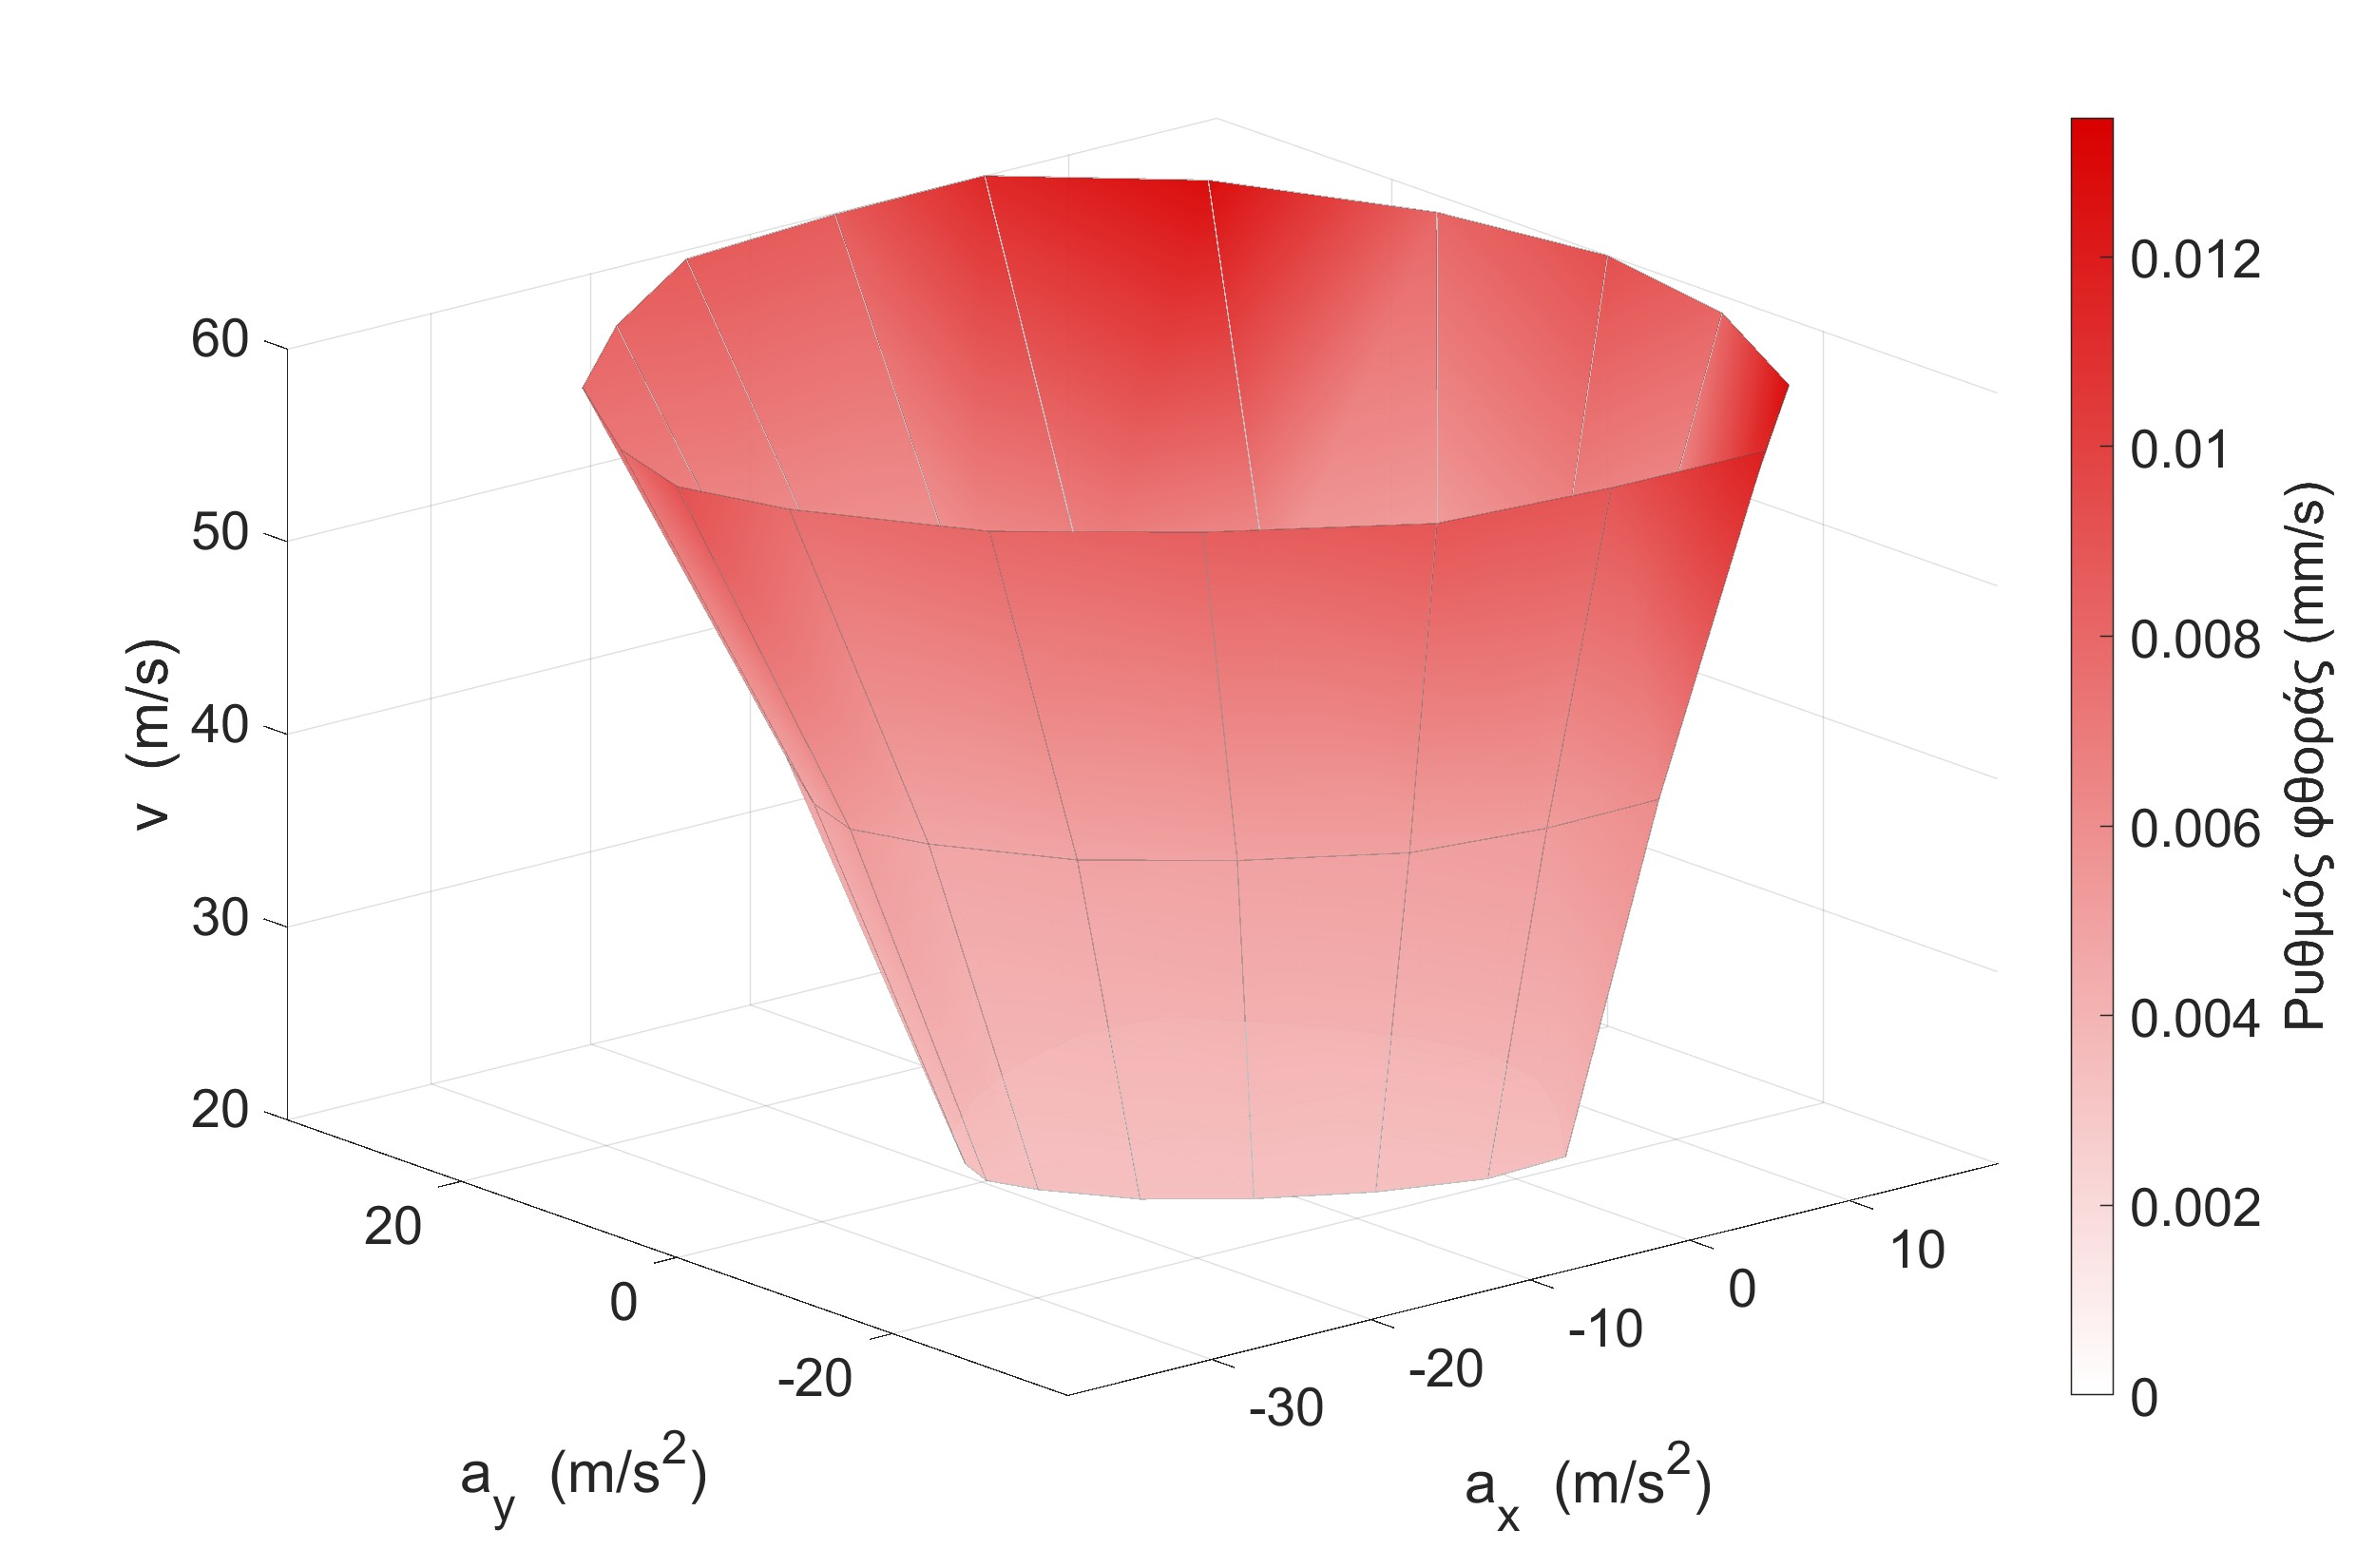
\includegraphics[width=0.85\textwidth]{figures/GGV_wearRate_110C.jpg}
    \caption{Διάγραμμα επιδόσεων στα $T_{\rm tyre}=110\,^\circ\mathrm{C}$, με χρώμα τον
    συνολικό ρυθμό φθοράς και των τεσσάρων ελαστικών σε κάθε σημείο πλέγματος.}
    \label{fig:ggv_wear_rate_110}
\end{figure}

\FloatBarrier
